
\section{Electromagnetic Induction II}

Name \rule{2.0in}{0.1pt}\hfill{}Section \rule{1.0in}{0.1pt}\hfill{}Date
\rule{1.0in}{0.1pt}

\bigskip
\bigskip
\bigskip


\textbf{Introduction}.
In this lab, we'll take a further look at Faraday's Law, which says
that a changing magnetic field can produce an emf (that is, a voltage)
in a loop of wire.  Current will be supplied to a large coil (which is a 
series of loops of wire), resulting in a magnetic field.  
If the current were constant in time,
then a steady magnetic field would be produced.  Since we want to
produce a changing magnetic field, we supply the coil with {\it
alternating current}, that is, current that flows back and forth in
alternating directions, oscillating in a sine-wave fashion.  The
result is an ever-changing magnetic field, which induces an emf in
a separate small coil.

\textbf{Apparatus}

\begin{itemize}

\item one large wire coil

\item one small wire coil

\item two banana plug leads with alligator clips

\item voltage sensor

\item Pasco 750 Interface

\end{itemize}

{\bf Setup.} The apparatus should be wired up to the computer interface in the 
following way: The two ends of the large coil should be connected to the output
terminals on the right side of the interface (using the banana plug leads with 
alligator clips). These output terminals supply alternating current to the 
large coil. The two ends of the small coil should be connected to a voltage 
sensor, which is plugged into port A on the interface. Place the small coil in 
the center of the large coil. Both coils should be arranged horizontally (that 
is, with the axes pointing straight up and down). If you are not sure whether 
things are hooked up correctly, consult your instructor.

{\bf Activity 1: Qualitative predictions.} Suppose that the top graph on the 
last page of this experiment represents the current flowing through the large 
coil as a function of time. When $I$ is positive, that means current is 
flowing in one direction around the coil, and when $I$ is negative the current 
is flowing in the other direction. On the axes below the top graph, sketch the 
shapes of the following other quantities.
In each case, don't worry about the overall scale on the vertical axis;
just focus on the shapes of the graphs, and particularly the locations
of the peaks and valleys.  Hint: some of the graphs will be exactly
the same shape as the given graph of $I$.

\begin{enumerate}
\item
On the first set of axes, sketch the vertical component of the magnetic field,
$B_z$, at the center of the large coil (realizing that this field is directly
proportional to the current in the coil).
\item On the the next set of axes, sketch the magnetic flux $\Phi_ B$ passing
through the small coil. (This flux is proportional to the magnetic field 
produced in the large coil).
\item On the bottom set of axes, sketch the emf ${\cal E}$ induced in the small
coil (which, by Farady's law, is proportional to the negative time derivative 
of the flux through the coil).
\end{enumerate}

The computer will measure and graph
$I(t)$, the current in the large coil, and ${\cal E}(t)$,
the emf in the small coil.  We want to test whether the two graphs are related
to each other in the way you predicted.  To be specific, make the following
predictions from your graphs before trying the experiment:

\newpage

\begin{enumerate}
\item At times when $I(t)$ is at its maximum value, what is ${\cal E}$?
\vskip .8in
\item At times when $I(t)$ is at its minimum value, what is ${\cal E}$?
\vskip .8in
\item At times when $I(t)=0$, what is ${\cal E}$?
\vskip .8in
\end{enumerate}

\bigskip\bigskip

{\bf Activity 2: Testing the predictions.}

Start the program called ``induction2.'' You should see two graphs,
one showing the current in the large coil and one showing the emf (voltage)
across the small coil.  Both graphs will be blank until you start taking
data, of course.  There should be an additional box that allows you to control
the frequency of oscillation of the alternating current.  Leave this alone
for now; we'll mess around with it later.

Hit ``Start'' and take data for about 5 seconds.  Do the shapes of the
two graphs generally match your predictions from Activity 1? (To answer this, you may want to expand the scales of the horizontal axes of the graphs so you can see the shapes better, and also align the graphs so that the times are synchronized.) 

\vskip 1in

If the answer to this question is ``yes,'' then go on.  If it's ``no,
the shape of the second one is exactly the opposite of what I expected,''
then you just have the small coil upside-down.  Turn it over and 
try again.  If the answer is not one of those two, then consult your 
instructor.

Let's be a bit more specific in comparing the predictions
with the data.  Examine the current graph, and record the
times of the first four moments when the current reaches a maximum.
Then look at the other graph, and record the emf at those same four times.
Are the results consistent with your prediction number 1 in Activity 1?

\newpage

Perform a similar analysis to check your predictions 2 and 3 from Activity 1.
In each case, check several appropriately-chosen moments of time to see
if the relationship between $I$ and ${\cal E}$ is as you predicted.

\vskip 4in

Suppose that you rotate the small coil 90$^\circ$, so that its axis
is horizontal.  What do you predict about the resulting emf?
Test your prediction and record the results here.

\newpage

\begin{center}

{\bf Graphs for Activity 1}

\vfil

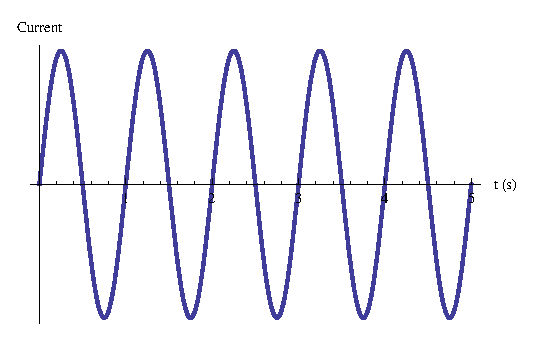
\includegraphics[width=2.9in]{indfig1.eps}

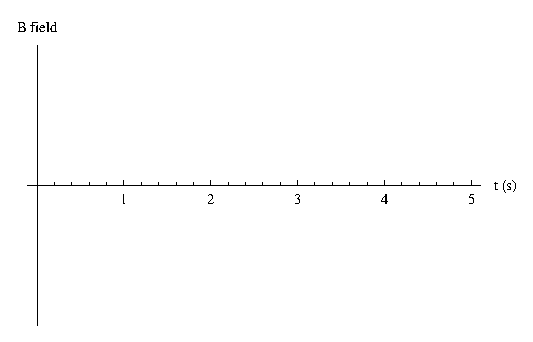
\includegraphics[width=2.9in]{indfig2.eps}

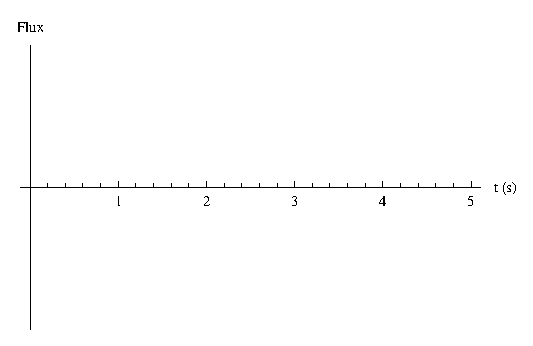
\includegraphics[width=2.9in]{indfig3.eps}

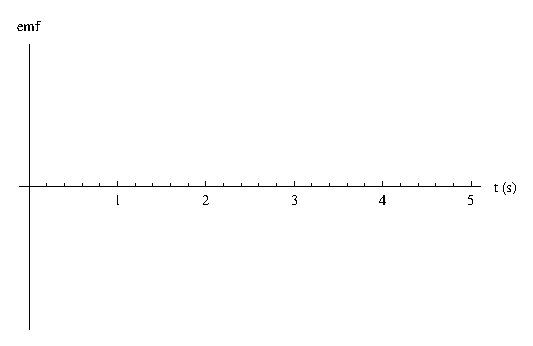
\includegraphics[width=2.9in]{indfig4.eps}



\vfil

\end{center}


